% \Huge

With the tools developed in the previous chapter, and the perfect reconstruction serving as an upper limit for reconstruction, we are ready to dive into realistic reconstruction methods. In Chapter 2 we outlined \todo{hopefully} many reconstruction methods used in practice, based on both Standard Perturbation Theory and Lagrangian Perturbation Theory. In this project, we base our reconstructions on the first order approximation to LPT (the Zel'dovich Approximation).

\section{The Zel'dovich reconstruction}

The key ingredient that we will use to perform realistic reconstructions is the density field. The idea behind the Zel'dovich approximation is to calculate a linear displacement field (we refer this field as Zel'dovich offset) based on the current peculiar velocities while taking into account the Hubble flow (see Chapter 2). \textit{Pynbody} has tools for calculating the Zel'dovich offset using the particle velocities in a snapshot. This offset is given by: \todo{ref???}

\begin{equation}
    \Psi_z(\textbf{q}) = (1+z) \times \textbf{v}(\textbf{q}) \times \frac{D(z)}{f(z)}
    \label{eq:4.1}
\end{equation} 

Where $D(z)$ is the linear growth factor, $f(z)$ is the rate of linear growth and $\textbf{v}(\textbf{q})$ is the velocity field. 

As we are interested in looking at the correlation between the reconstructed field  and the initial fields in our simulations (which are at $z=99$), we need to calculate the Zel'dovich offset up to $z=99$ only. In order to achieve this, we first used equation~\ref{eq:4.1} to calculate the offset starting from the redshift $z$ of the snapshot ($\Psi_z$). After that, we used the same equation to approximate this offset from $z=99$ ($\Psi_{99}$) using the same velocity field. The displacement field we are after is then given by:

\begin{equation}
    \Psi(\textbf{q}) = \Psi_z(\textbf{q}) - \Psi_{99}(\textbf{q})
    \label{eq:4.2}
\end{equation}
 
We first start out in our investigation by performing a reconstruction using the Zel'dovich offset calculated directly from the particle velocities in each snapshot. The methodology of the reconstruction resembles the Perfect Reconstruction. We first calculate the density field at the particle positions in a snapshot, and then we apply the Displacement field $\Psi(\textbf{q})$ to move the particles. The density field is carried along. After that, \textsc{GenPK} is used to measure the cross power-spectra of the reconstructed field with the initial ($z=99$) field.

\begin{figure}
    \centering
    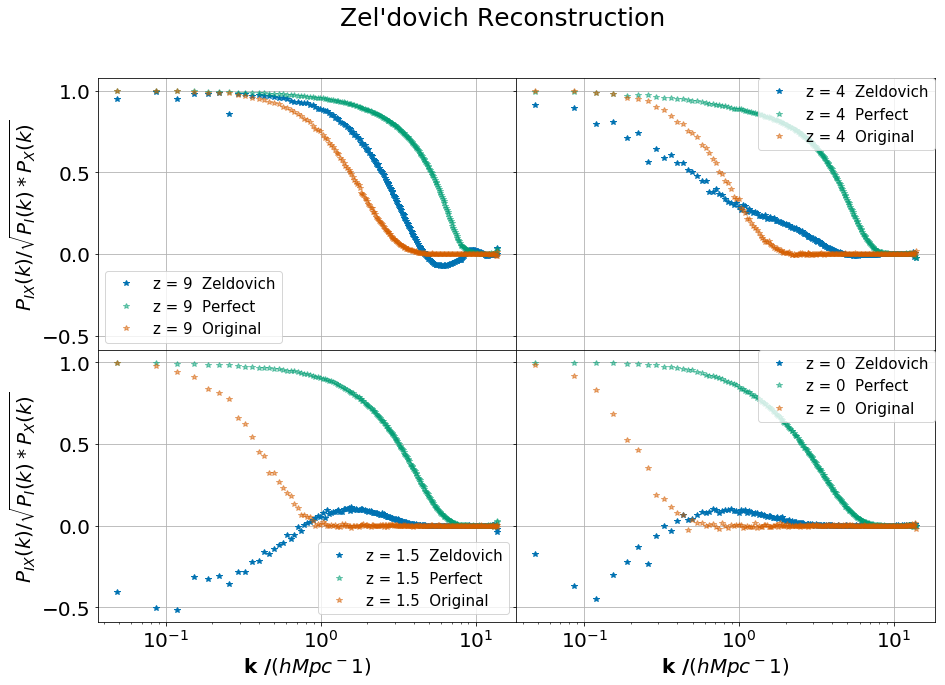
\includegraphics[width=1\columnwidth]{images/realRecon/zeld.png}%
    
    \caption{
    Normalized cross-spectra between the Zel'dovich reconstruction and the initial field. This reconstruction was performed by linearly moving the particles back in time (using the Zel'dovich approximation). As we apply the linear approximation directly to the particle velocities, this gives a good indicator of the regime we are in at that redshift. We see the reconstruction work very well when starting from $z=9$, which indicates we are still in the quasi-linear regime there. However, as time progresses (lower redshift) the correlation breaks down even on the largest scales, indicating we are mostly in the non-linear regime. 
    }
    
    \label{fig:4.1}
\end{figure}

The results of this reconstruction (we call it the Zel'dovich reconstruction) can be seen in~\ref{fig:4.1}. We again look at the normalized cross-spectra between this reconstruction and the initial density field. To give us a better understanding of how well this method works, the original correlation and the perfect reconstruction are also present. The figure presents the reconstruction starting from four different snapshots in the redshift interval $z=9$ to $z=0$.

The reconstruction starting at $z=9$ gives very good results, bringing the decorrelation scale to an intermediate step between the original and the perfect reconstruction. At this redshift most particles are still in the quasi-linear regime, so this result was expected. An interesting feature is the small anti-correlation obtained at large $k$. This effect is most likely due to particles in non-linear regimes which are past shell-crossing. To understand what gives rise to this anti-correlation, consider two fronts of matter collapsing towards each other. After shell crossing \todo{this should be explained in chapter 2.} there will be a turn-around as the two evolve into a single filament. If we linearly track these velocities back, we are effectively going the wrong way. This will lead to an anti-correlation over the affected scales. For the $z=9$ reconstruction, this effect is very small, indicating that shell crossing has only occurred on the smallest scales, and that most particle motions can be well approximated with the linear regime. 

However, starting from lower redshifts produces results much worse than even the original. This was expected, as at these redshifts most particles are now in the non-linear regime. By still treating their motions as linear we are breaking even the correlation that was there to begin with. Figure~\ref{fig:4.1} shows the largest scales decorrelating as we move to reconstructions from lower redshifts, and even leading to anti-correlation. For the lowest redshifts, we see a small improvement in the correlation on intermediate scales, but anti-correlation on large scales. This result is much harder to understand. A possible explanation is an extension to the reasons presented above for the small scales in the $z=9$ reconstruction. The effect of anti-correlation due to particles that are past shell crossing moving the wrong way within the Zel'dovich approximation is expected to increase with decreasing redshift. This might lead to the large scales also becoming anti-correlated. This effect should be studied further, however, we leave this for future works, as our aim in this project is to achieve a good reconstruction.

The Zel'dovich approximation is then not a good reconstruction method at low redshift when most particles have non-linear velocities. For these regimes we need higher orders of LPT to perform the reconstruction. However, at this point it is hard to justify this pursuit from an observational stand point. In this section we have used the peculiar velocities of particles in our simulations. As the ultimate goal of any reconstruction technique is to be used in practice on real data, we need to consider the feasibility of our method. Observers usually detect a few galaxies over an $8-10$ Mpc scale\todo{find ref}, and any peculiar velocity measurement inevitably come with errors. This means that the Zel'dovich reconstruction we just performed is very unrealistic in practice. The goal of the rest of this chapter is to modify the Zel'dovich reconstruction to make it more realistic, and also to improve its performance at low redshift.

\section{Getting back to the linear regime}

In order to make the Zel'dovich approximation work for our reconstruction, we must somehow get back into the linear regime. As discussed in Chapter 2, matter tends to be collapsed into filaments at late times. This means individual particles have non linear velocities, but ensembles of particles might still be in the linear regime. Our solution to the two problems outlined in the previous section is to use bulk velocities to calculate the Zel'dovich offset, instead of individual particle velocities.

We smooth particle velocities over 1 Mpc and 10 Mpc scales respectively before calculating the Zel'dovich offset. This means we are now considering bulk motions instead of particle motions. These bulk motions will hopefully provide a better start point when we calculate the Zel'dovich offset. The other effect of this smoothing is that it makes this method more realistic. With the technology we currently have, observers can maybe detect a few galaxies in a 10 Mpc bin\todo{ref}, so by smoothing our velocity field over that scale, we simulate a more realistic scenario. The reason for also attempting a separate reconstruction using velocities smoothed over 1 Mpc scales is twofold. Firstly, we want to understand the effect of the velocity smoothing scale on the reconstruction. Secondly, we use the 1 Mpc case as a test for what could be achieved with improving technology and a better handling of systematics which could be useful for the next generation of Galaxy Surveys.

To perform these reconstructions, we first split a simulation into bins of a given size: $(1 Mpc)^3$ or $(10 Mpc)^3$. We then use the positions of the particles to identify the bin they are in. After that, an average velocity over the particles in each bin is calculated. This average velocity is assigned to the centre of the bin. In this manner, we construct a three-dimensional grid which contains a measure of the average velocity field. Finally, we use this average velocity field to linearly interpolate the value of the velocities at the particle positions. In this manner, velocities are smoothed over the scales of interest. Using these new velocities, the Zel'dovich reconstruction is performed as outlined in the previous section. 

Before we move on to the results, an interesting side effect that should be mentioned showed up during the reconstruction. The nature of our method implies that we are creating coherent movements of particles. This coherent movement leaves large gaps in our reconstructed density field (regions where the density field is equal to 0). These gaps become a problem when we want to take the logarithm of the density field as discussed in Chapter 3. When calculating the density field, \textit{Pynbody} uses a smoothing kernel which normally fills in these gaps. However, this method uses N nearest neighbours to calculate the smoothing scale in a region. Normally, there still are a few particles even in the largest voids. These particles will have very far away neighbours, imposing a large smoothing scale. On the other hand, by creating coherent movements, completely empty regions arise. Particles on the edges of these empty regions can easily find nearby neighbours and establish a relatively small smoothing scale. Our solution is to manually find these empty regions and assign a very small value to the density field. 

\section{Results}

The first step is to investigate the impact of the smoothing scale.

\begin{figure}
    \centering
    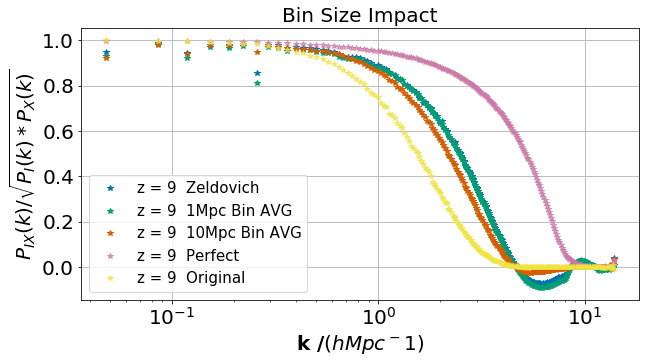
\includegraphics[width=1\columnwidth]{images/realRecon/binSize.png}%
    
    \caption{
    Normalized cross-spectra of realistic reconstructions with the initial field. This figure shows the impact of smoothing velocities over certain scales. Because we lose information by smoothing, the 10 Mpc reconstruction recovers less information compared to the 1 Mpc reconstruction. The Zel'dovich reconstruction is also present for comparison. It's proximity to the 1 Mpc reconstruction might indicate that smoothing velocities over this scale is not enough to get back into the linear regime. However, as we are looking at reconstructions from $z=9$, they all work quite well because most particles are still in the quasi-linear regime.
    }
    
    \label{fig:temp}
\end{figure}


% \begin{figure}
%     \centering
%     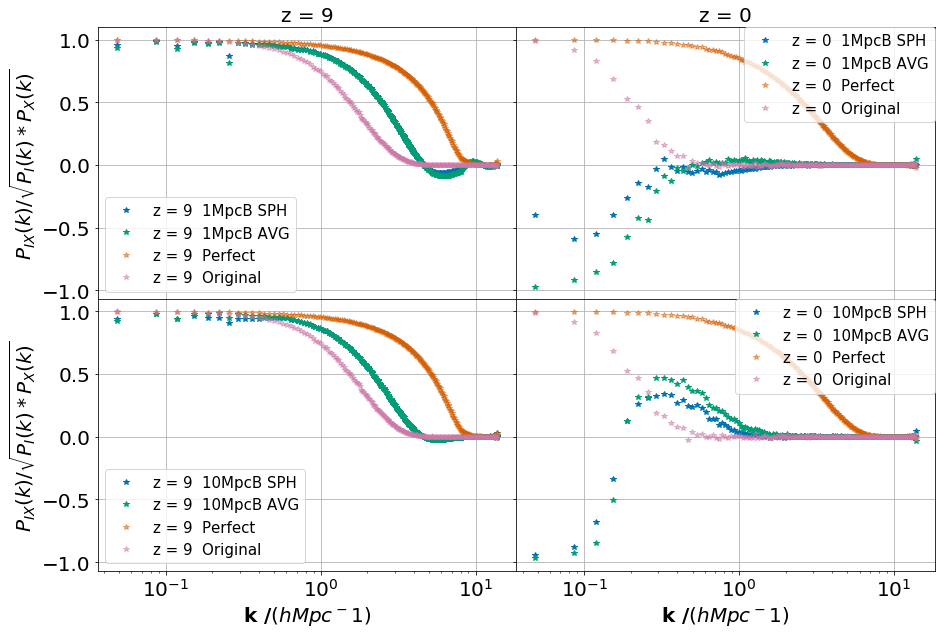
\includegraphics[width=1\columnwidth]{images/realRecon/sphVsAvg.png}%
    
%     \caption{
%     Cross spectra of realistic reconstructions from redshift 9 and 0, using 1 Mpc and 10 Mpc bins to average velocities. There are two averaging methods used: AVG - average of all particles in each bin, SPH - A point estimate of the velocity at the center of the bin.  
%     }
    
%     \label{fig:8}
% \end{figure}

\begin{figure}
    \centering
    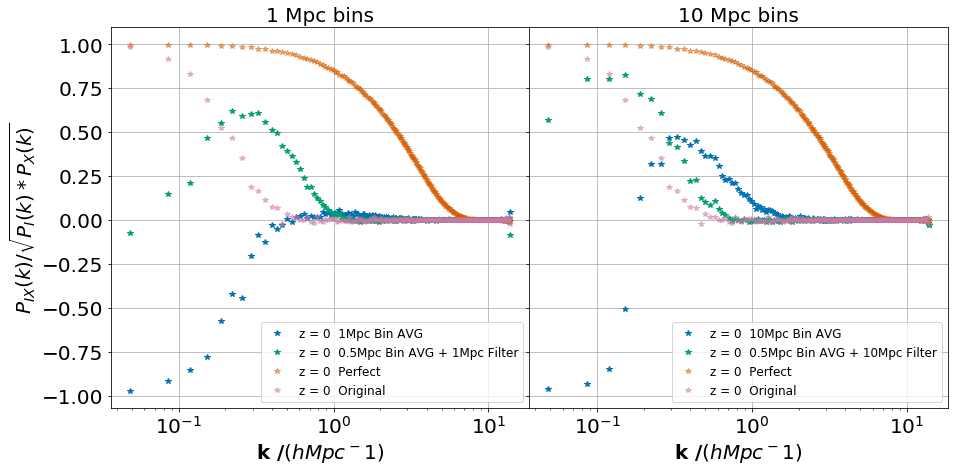
\includegraphics[width=1\columnwidth]{images/realRecon/filterComp.png}%
    
    \caption{
        Cross spectra of realistic reconstructions from redshift 9 and 0, using 1 Mpc and 10 Mpc bins to smooth velocities. Filter -no filter comparison
    }
    
    \label{fig:9}
\end{figure}


\section{Analysis}

\todo[inline]{Talk about the results for different averaging methods and Bin Sizes.}

\begin{figure}
    \centering
    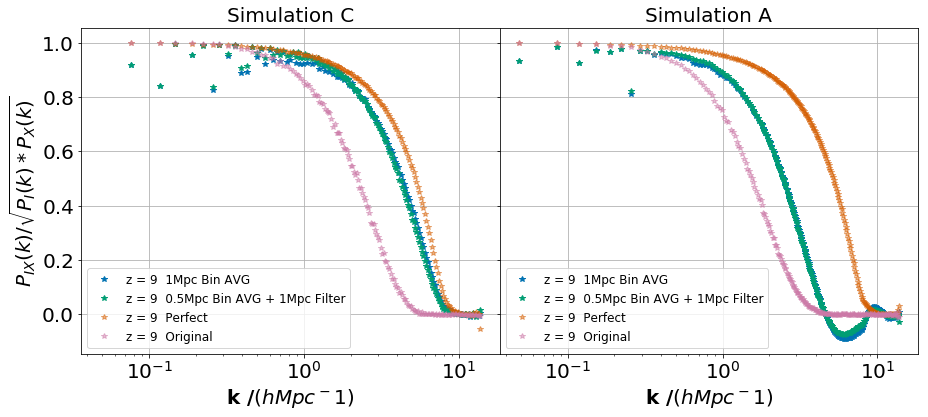
\includegraphics[width=1\columnwidth]{images/realRecon/z9SimComp.png}%
    
    \caption{
        Z9 comparison
    }
    
    \label{fig:10}
\end{figure}

\begin{figure}
    \centering
    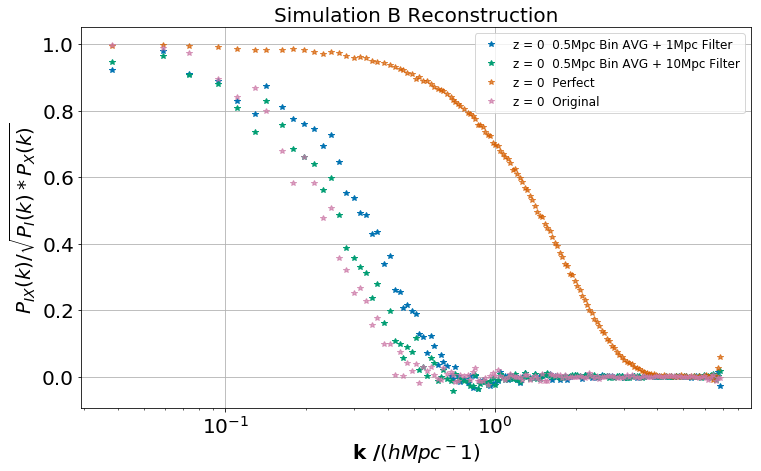
\includegraphics[width=1\columnwidth]{images/realRecon/simBRecon.png}%
    
    \caption{
        Simulation B reconstruction
    }
    
    \label{fig:11}
\end{figure}

\begin{figure}
    \centering
    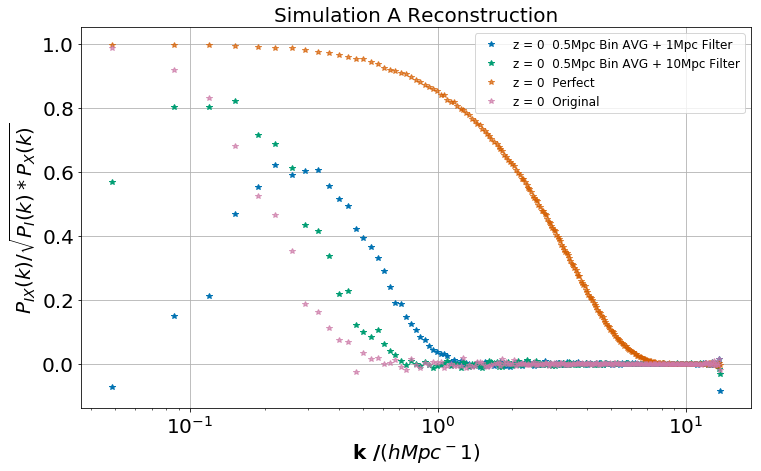
\includegraphics[width=1\columnwidth]{images/realRecon/simARecon.png}%
    
    \caption{
        Simulation A reconstruction
    }
    
    \label{fig:12}
\end{figure}